\documentclass[abstract=on,10pt,a4paper,bibliography=totocnumbered]{article}
\usepackage[paper=a4paper,left=35mm,right=35mm,top=25mm,bottom=30mm]{geometry}
\usepackage[doublespacing]{setspace}
\usepackage[english]{babel}
\usepackage[utf8]{inputenc}
\usepackage[round]{natbib}
\usepackage{amsmath}
\usepackage{colortbl}
\usepackage{amsfonts}
\usepackage{amssymb}
\usepackage{gensymb}
\usepackage{graphicx}
\usepackage{tikz}
\usepackage{enumerate}
\usepackage{enumitem}
\usepackage{subcaption}
\usepackage{booktabs}
\usepackage[hidelinks]{hyperref}
\usepackage[nameinlink]{cleveref}
\usepackage{lineno}
\usepackage{multirow}
\usepackage{arydshln}
\usepackage[nomarkers, nolists]{endfloat}

%------------------------------------------------------------------------------
%	Some Styling
%------------------------------------------------------------------------------
% Creating some TikZ styles
\tikzset{
  nonterminal/.style = {rectangle
    , minimum size = 6mm
    , very thick
    , draw = black!
  }
}

% Changing the style of captions in figures etc.
\captionsetup{labelfont=bf, format=plain, font=small}

% Change how equations are referenced
\renewcommand{\theequation}{Equation \arabic{equation}}%

%------------------------------------------------------------------------------
%	Titlepage: Header
%------------------------------------------------------------------------------
\title{Bound within Boundaries: How Well Do Protected Areas Match Movement
Corridors of Their Most Mobile Protected Species?}

% List of Authors
\author{
  David D. Hofmann\textsuperscript{1,\S,*} \and
  Dominik M. Behr\textsuperscript{1,2,*} \and
  John W. McNutt\textsuperscript{2} \and
  Arpat Ozgul\textsuperscript{1} \and
  Gabriele Cozzi\textsuperscript{1,2}
}

% Reduce spacing between authors
\makeatletter
\def\and{%
  \end{tabular}%
  \hskip -0.5em \@plus.17fil\relax
  \begin{tabular}[t]{c}}
\makeatother

% Current Date
\date{\today}

% And here the masterpiece begins
\begin{document}

% Change page numbering
\pagenumbering{gobble}

% Required to be able to cite
\bibliographystyle{apalike}

% Create Titlepage
\maketitle

%------------------------------------------------------------------------------
%	Titlepage: Additional Info
%------------------------------------------------------------------------------
\begin{flushleft}

\vspace{0.5cm}

\textsuperscript{1} Department of Evolutionary Biology and Environmental
Studies, University of Zurich, Winterthurerstarsse 190, 8057 Zurich,
Switzerland.

\textsuperscript{2} Botswana Predator Conservation Trust, Private Bag 13, Maun,
Botswana.

\textsuperscript{\S} Corresponding author (david.hofmann2@uzh.ch)

\textsuperscript{*} Shared first authorship

\vspace{4cm}

\textbf{Running Title:} Connectivity across a Transfrontier Conservation Area.

\vspace{0.5cm}

\textbf{Keywords:} dispersal, habitat selection, integrated step selection
function, Kavango-Zambezi Transfrontier Conservation Area, landscape
connectivity, least-cost corridors, Lycaon pictus, permeability surface,
protected areas, wildlife management

\end{flushleft}

%------------------------------------------------------------------------------
%	Abstract
%------------------------------------------------------------------------------
\newpage
\begin{abstract}
\noindent 1. Conserving and managing large portions of land to connect wildlife
reserves is increasingly used to maintain and restore connectivity among
wildlife populations. Boundaries of such conservation areas are often determined
based on expert opinion and socio-political constraints, yet the extent to which
they match species' movement corridors is rarely examined. This is mainly due to
a lack of data, particularly on wide-ranging movement behavior such as
dispersal. Nevertheless, empirically assessing the adequacy of protected areas
is key for the implementation of targeted management actions and efficient use
of limited conservation funds.

\noindent 2. Between 2011 and 2019, we collected high-resolution GPS movement
data on 16 dispersing African wild dog (\textit{Lycaon pictus}) coalitions from
a free-ranging population in the Kavango-Zambezi Transfrontier Conservation Area
(KAZA-TFCA). Spanning five countries and 520'000 km\textsuperscript{2} the
KAZA-TFCA is the world's largest transboundary conservation area and a prime
example for international conservation efforts. We used integrated step
selection analysis to estimate habitat preferences of dispersers and to create a
permeability surface for the entire KAZA-TFCA. We compared landscape
permeability across different regions within the KAZA-TFCA as well as outside
its boundaries. Lastly, we calculated least-cost paths and corridors to verify
that major movement routes were adequately encompassed within the KAZA-TFCA.

\noindent 3. Permeability within the boundaries of the KAZA-TFCA was more than
double compared to areas outside it. Furthermore, we observed a five-fold
permeability difference among the five KAZA-TFCA countries. We further showed
that major movement corridors of wild dogs run within the KAZA-TFCA, although
some minor routes remained outside formally protected areas.

\noindent 4. Differences in permeability were mainly caused by different degrees
of human activities across regions, which hampered dispersal. Rivers, swamps  or
open water also limited dispersal, while other landscape features had a limited
effect.

\noindent 5. \textit{Synthesis and Applications}: In this study, we showed how
pertinent dispersal data of a highly mobile species can be used to empirically
evaluate the adequacy of already-existing or planned protected areas.
Furthermore, observed regional differences in landscape permeability highlight
the need for a coordinated effort towards maintaining or restoring connectivity,
especially where international effort is required.
\end{abstract}

%------------------------------------------------------------------------------
%	Main Text
%------------------------------------------------------------------------------
\newpage

% Change page numbering
\pagenumbering{arabic}

% Create linenumbers
\linenumbers

\section{Introduction}
Connectivity among subpopulations is a crucial pre-requisite for many species to
thrive and persist \citep{Fahrig.2003}. Accordingly, preserving and protecting
movement corridors between wildlife reserves has become an utmost task for
conservation management \citep{Doerr.2011, Rudnick.2012}, resulting in an
ever-growing number of large and often transboundary protected areas. While
boundaries of such areas are often drawn according to expert opinion and
socio-political needs, subjective assessments have revealed deficiencies in the
past \citep{Clevenger.2002, Pullinger.2010}. Thus, an empirical assessment of
the adequacy of already-existing or planned protected areas using pertinent
animal movement data is paramount for targeted use of valuable and scarce
conservation funds \citep{Pullinger.2010}.

In recent years, a growing body of research has used animal relocation data to
identify movement corridors and assess connectivity at large scales (e.g.
\citealp{Chetkiewicz.2006, Squires.2013, Elliot.2014}). Identification of
potential corridors typically relies on the estimation of permeability surfaces,
which return the ease or willingness at which the focal species traverses a
specific landscape \citep{Sawyer.2011}. Such surfaces are created based on a
species' habitat preferences, which can be quantified using a suite of selection
functions \citep{Zeller.2012}. Specifically, habitat preferences are estimated
by comparing spatial covariates (e.g. environmental and anthropogenic) at
locations visited by the animal to the same spatial covariates at randomly
selected locations \citep{Zeller.2012}. Importantly, selection functions rely on
adequate landscape and relocation data that are representative of the process
being studied \citep{Diniz.2020}. For instance, relocation data collected on
dispersing individuals has been shown to outperform data collected on resident
individuals in the detection of large-scale movement corridors
\citep{Elliot.2014, Diniz.2020}. Nevertheless, dispersal data is inherently
difficult to collect and remains scarce in the connectivity literature
\citep{Vasudev.2015}. As such, most permeability surfaces upon which movement
corridors are identified are created using relocation data collected on resident
individuals. This introduces severe biases and substantially reduces the power
to reveal meaningful movement corridors, for dispersing individuals have
different needs and drives compared to resident individuals \citep{Elliot.2014,
Cozzi.2020}. Such biases have limited our ability to meaningfully assess the
effectiveness of protected areas in securing connectivity for their protected
species.

One initiative that aims at restoring and enhancing connectivity across large
scales is the Kavango-Zambezi Transfrontier Conservation Area (KAZA-TFCA), which
constitutes the world's largest transfrontier conservation area, spanning over
520'000 km\textsuperscript{2} and five countries (\url{www.kavangozambezi.org}).
While the KAZA-TFCA was originally set to facilitate movements of African
elephants (\textit{Loxodonta africana}; \citealp{Tshipa.2017}), it is also key
to the conservation of other wide-ranging species such as African wild dogs
(\textit{Lycaon pictus}; \citealp{Woodroffe.2012, Cozzi.2020}), lions
(\textit{Panthera leo}; \citealp{Elliot.2014, Cushman.2018}), and cheetahs
(\textit{Acinonyx jubatus}; \citealp{Weise.2017}). To date, however, few studies
have attempted to assess the adequacy of the KAZA-TFCA using relevant global
positioning system (GPS) relocation data of its protected species at the
appropriate spatial scale \citep{Elliot.2014, Tshipa.2017}. Thus, how well the
boundaries of the KAZA-TFCA reflect natural movement patterns and dispersal
corridors of its most mobile protected species is virtually unknown.

Across the KAZA-TFCA, the African wild dog (\textit{Lycaon pictus}) represents a
highly mobile and endangered flagship species for conservation efforts. Once
widespread across the entire Sub-Saharan continent, wild dogs have been widely
extirpated through human persecution, habitat destruction, and disease outbreaks
\citep{Woodroffe.2012}. As a result, the species has become one of Africa's most
endangered large carnivores, and currently only survives in small, spatially
scattered subpopulations \citep{Woodroffe.2012}. Within these subpopulations,
wild dogs form cooperative breeding packs of up to thirty individuals
\citep{Creel.2002}, whose social structure is strongly governed by the process
of dispersal \citep{McNutt.1996, Behr.2020}. Both males and females disperse
from their natal pack, either alone or in same-sex dispersing coalitions, and
search for unrelated mates and a suitable territory to settle
\citep{McNutt.1996, Cozzi.2020, Behr.2020}. During dispersal, wild dogs can
cover several hundred kilometers \citep{Masenga.2016, Woodroffe.2019,
Cozzi.2020}. Despite the importance of dispersal for the long-term viability of
this species, little empirical information is available on habitat selection and
potential movement barriers during dispersal. The few studies that have
collected dispersal data have shown that dispersers quickly move over large
distances, avoid human-dominated landscapes and areas densely covered by trees,
but prefer proximity to water \citep{Masenga.2016, Woodroffe.2019, Oneill.2020,
Cozzi.2020}.

Here, we collected GPS relocation data on 16 dispersing wild dogs in as many
dispersing coalitions from a free-ranging population in northern Botswana and
analyzed it to assess the adequacy of the KAZA-TFCA in securing connectivity. We
estimated the degree of selection or avoidance for environmental and
anthropogenic landscape features and used the obtained habitat preferences to
predict a permeability surface spanning the entire KAZA-TFCA. We then
investigated how landscape permeability varies regionally and internationally
and compared permeability within and outside the KAZA-TFCA boundaries. Finally,
we calculated least-cost paths and corridors to identify major movement routes
and to verify that these are successfully covered by the KAZA-TFCA.

\section{Methods}
\subsection{Study Area}
The study area (centered at -17\degree 13'9''S, 23\degree 56'4''E;
\Cref{StudyArea}a) was outlined by a rectangular bounding box stretching over
1.3 Mio km\textsuperscript{2} and encompassing the entire KAZA-TFCA
(\Cref{StudyArea}b). The KAZA-TFCA lies in the basins of the Okavango and
Zambezi rivers and includes parts of Angola, Botswana, Namibia, Zimbabwe, and
Zambia. With a total area of over 520'000 km\textsuperscript{2} it constitutes
the earth's largest transboundary conservation area and is characterized by
diverse landscapes, including savanna, grassland, and dry or moist woodland
habitats. Rainfall in the study area is seasonal and lasts from November to
March. The KAZA-TFCA also comprises the Okavango Delta, which represents a
highly dynamic hydrological flood-pulsing system \citep{McNutt.1996,
Wolski.2017}. The extent of the flood in the delta greatly changes within and
between years depending on the amount of rain that descends from the catchment
areas in Angola and reaches the distal ends of the delta between July and August
(Figure S4). The flood drastically affects surrounding landscapes, so that
during maximum extent (ca. 12'000 km\textsuperscript{2}) the delta becomes a
patchy conglomerate of swamps, open water, and islands, whereas these structures
run dry when the flood retracts to its minimum extent (ca. 5'000
km\textsuperscript{2}; \citealp{Wolski.2017}). Despite 36 national parks (NPs)
and other protected areas, there is considerable human influence in some regions
of the KAZA-TFCA, mainly originating from farms, high human density, and road
traffic.

\begin{figure}[h]
  \begin{center}
    \begin{tikzpicture}
        \node[anchor=south west,inner sep=0] (image) at (0,0,0) {
        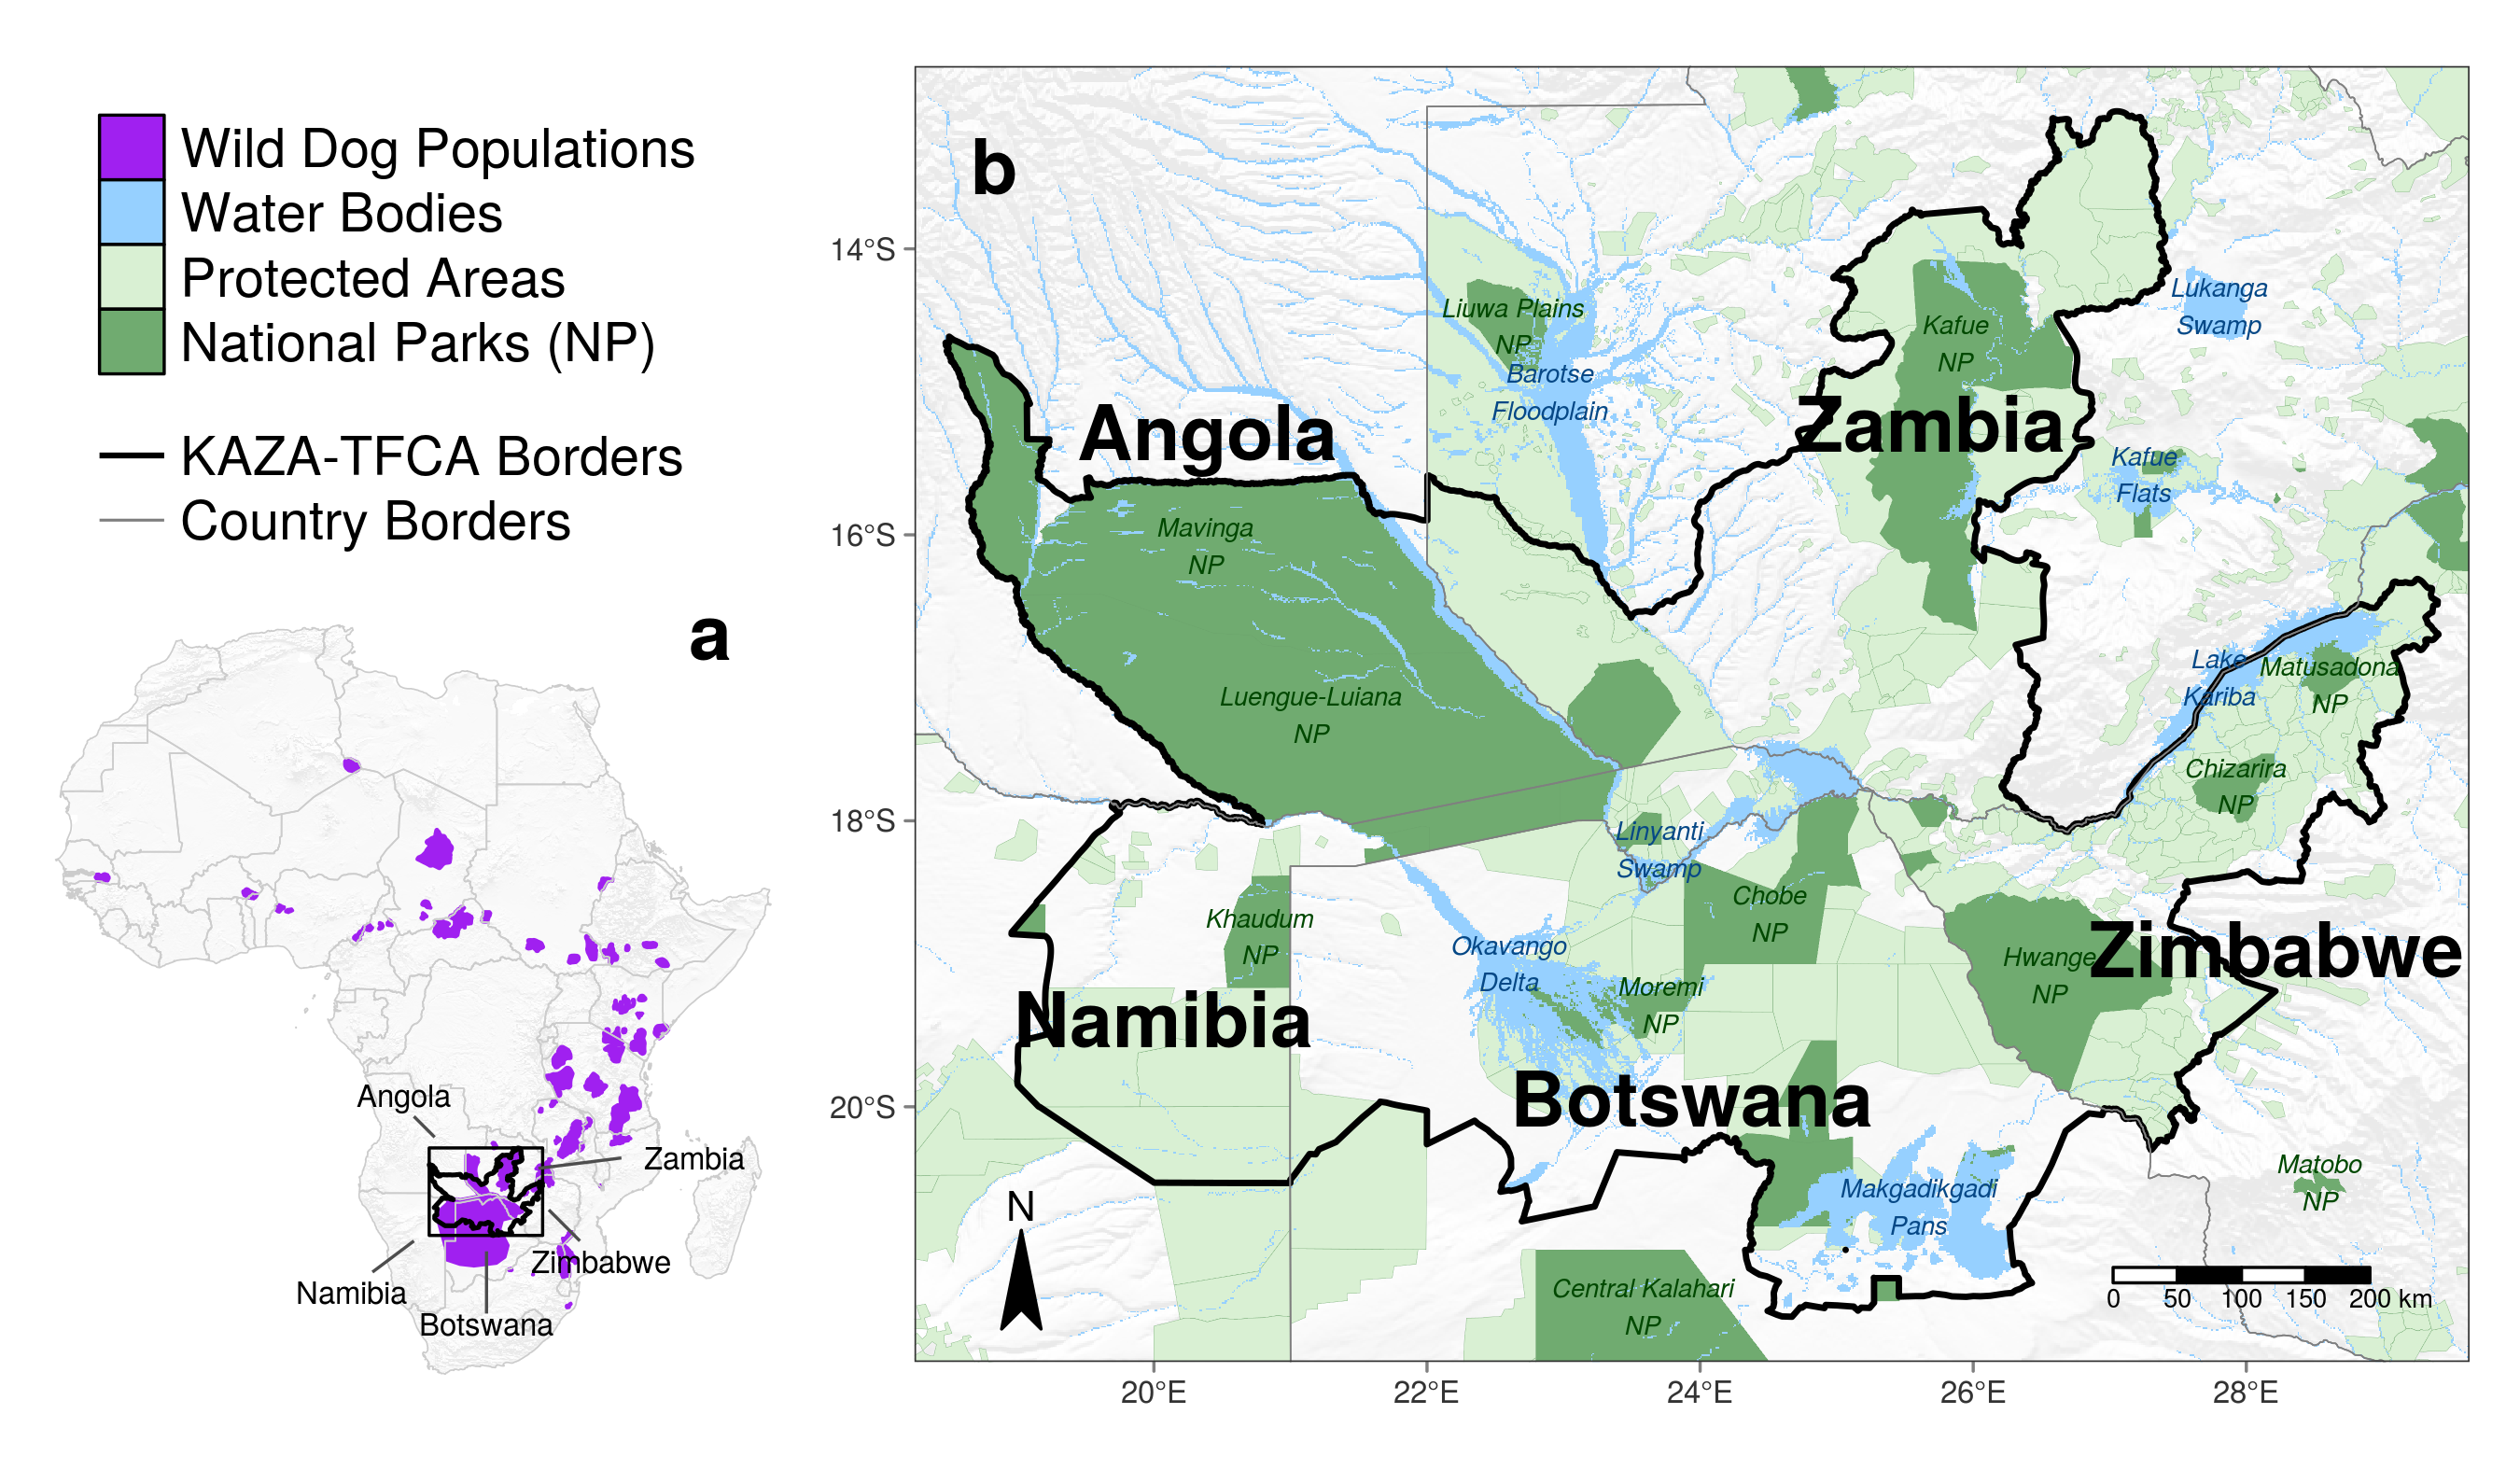
\includegraphics[width=\textwidth]{99_StudyArea.pdf}
        };
        \begin{scope}[x={(image.south east)},y={(image.north west)}]
            % % next four lines will help you to locate the point needed by forming a grid.
            % % comment these four lines in the final picture.
            % \draw[help lines,xstep=.1,ystep=.1] (0,0) grid (1,1);
            % \draw[help lines,xstep=.05,ystep=.05] (0,0) grid (1,1);
            % \foreach \x in {0,1,...,9} { \node [anchor=north] at (\x/10,0) {0.\x}; }
            % \foreach \y in {0,1,...,9} { \node [anchor=east] at (0,\y/10) {0.\y};}
            % % upto here
            \draw[black] (0.202, 0.255) -- (0.36, 0.955);
            \draw[black] (0.202, 0.205) -- (0.36, 0.070);
        \end{scope}
    \end{tikzpicture}
    \caption{Overview of our study area. (a) The red dotted rectangle depicts
    the study area, which was confined by a bounding box encompassing the entire
    KAZA-TFCA. Gray areas indicate remaining wild dog populations according to
    the IUCN \citep{Woodroffe.2012}. (b) The white rectangle illustrates the
    area within which dispersing coalitions were collared. Since Game Reserves
    in Botswana virtually serve the same purpose as National Parks, we use the
    terms interchangeably for this region.}
    \label{StudyArea}
  \end{center}
\end{figure}

\subsection{GPS Relocation Data}
We used a population of free-ranging African wild dogs inhabiting the Okavango
Delta in northern Botswana as a source population for dispersing individuals.
This population has been extensively studied since 1989 \citep{McNutt.1996,
Cozzi.2013, Cozzi.2020, Behr.2020}. Between 2011 and 2019, we systematically
collected GPS relocation data on 16 coalitions of dispersing African wild dogs
(7 female and 9 male coalitions). Candidate dispersing individuals were
identified based on criteria reported in \cite{Behr.2020}, immobilized according
to protocols described in \cite{Osofsky.1996}, and fitted with GPS/Satellite
radio collars (\textit{Vertex Lite; Vectronic Aerospace GmbH, Berlin}) while
still with their natal pack. All procedures were undertaken and supervised by a
Botswana-registered wildlife veterinarian. During dispersal, GPS collars were
programmed to record GPS relocation data every 4 hours and to regularly transmit
them via Iridium satellite system to a base station.

Because we were interested in dispersal behavior only, we discarded any GPS data
collected while individuals were still with their natal packs and after
settlement in a new territory \citep{Cozzi.2020}. We identified the exact time
of emigration and settlement based on direct field observations and through
visual inspection of the net squared displacement (NSD) metric. NSD quantifies
the Euclidean distance of a relocation to a reference point \citep{Borger.2012},
which in our case was the center of the dispersing coalition's natal home range.
Thus, dispersal was deemed to have started when a coalition had left its natal
home range and continued until the NSD metric remained stationary, implying that
the coalition had successfully settled (Figure S1). In total, we collected 4'169
GPS relocations during dispersal (Figure S2 \& Table S1), resulting in an
average of 260 locations per dispersing coalition (min = 37, max = 729). In our
analysis, we did not differentiate between male and female dispersing
coalitions, for previous research found little differences between sexes during
dispersal \citep{Woodroffe.2019, Cozzi.2020}.

\subsection{Spatial Covariates}
To investigate habitat preferences of dispersing wild dogs, we used a set of
geo-referenced covariates (\Cref{Covariates}) that we aggregated in the
categories \textit{land cover} (which included water cover, distance to water,
shrubs/grassland cover, and tree cover), \textit{protection status} (protected
vs. unprotected), and \textit{human pressure} (which included human influence,
presence of roads, and distance to roads). For each of these covariates we
prepared spatial raster layers from freely available online services or from
remotely sensed satellite imagery. To ensure a consistent resolution (i.e.
cell-size or grain) across covariates, we coarsened or interpolated all layers
to match a resolution of 250m x 250m. For further details on the preparation of
each covariate, see Appendix A.3. We performed processing and manipulation of
data as well as all spatial and statistical analyses using R, version 3.6.1
\citep{R.2019}.

\begin{figure}[h]
  \begin{center}
    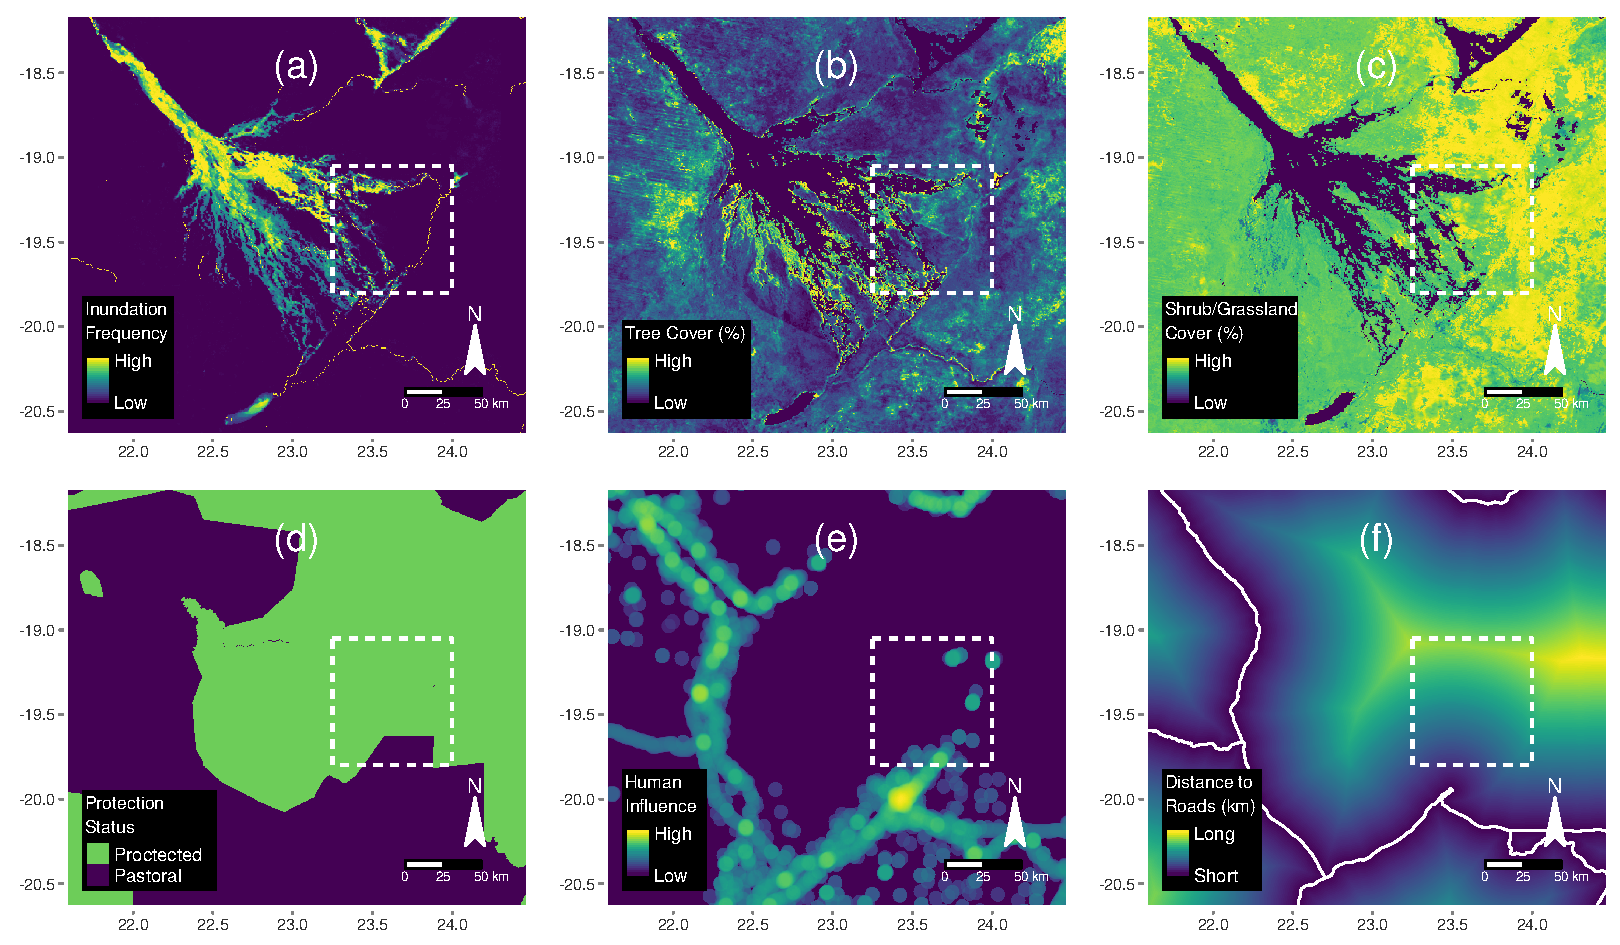
\includegraphics[width = \textwidth]{99_Covariates.pdf}
    \caption{Overview of spatial covariates that we included in our models. We
    prepared all covariates for the entire study area but for better visibility
    we only plot them for the surroundings of the Okavango Delta. The white
    rectangle in each plot depicts the area within which dispersing coalitions
    were collared. (a) Averaged layer of all dynamic (binary) water maps. (b)
    Percentage cover of trees. (c) Percentage cover of shrubs/grassland.
    Anything that was not covered by trees or shrubs/grassland was deemed to be
    bare land. (d) Protection status of the area. (e) Human influence proxy
    composed of human density, farms, and roads. (f) Distance to nearest road
    (white lines depict actual roads).}
    \label{Covariates}
  \end{center}
\end{figure}

\subsection{Habitat Selection Model}
We used an integrated step selection function (iSSF; \citealp{Avgar.2016}) to
investigate dispersers' selection or avoidance for the above-mentioned spatial
covariates. That is, we paired each realized step (i.e. the connecting line
between two consecutive GPS relocations; \citealp{Turchin.1998}) with 24 random
steps. We generated random steps by sampling turning angles from a uniform
distribution U(\(-\pi, +\pi\)) and step lengths from a gamma distribution that
was fitted using realized steps \citep{Avgar.2016}. A realized step and its 24
associated random steps formed a stratum that received a unique identifier.
Along each step, we extracted the above-mentioned covariates (Table S3),
standardized extracted values using a z-score transformation, and checked for
correlation using Pearson's Correlation Coefficient \(r\). None of the
covariates were overly correlated (\(|r| > 0.6\); \citealp{Latham.2011}) and we
retained all of them for modeling. Our habitat selection model then assumed that
dispersing wild dogs assigned a selection score \(w(x)\) of the following
exponential form to each realized and random step \citep{Fortin.2005}:

\begin{equation}
\label{EQ1}
  w(x) = exp(\beta_1 x_1 + \beta_2 x_2 + ... + \beta_n x_n)
\end{equation}

\noindent The selection score \(w(x)\) of a step depended on its associated
covariates (\(x_1, x_2, ..., x_n\)), as well as on the animal's preferences for
these covariates (\(\beta_1, \beta_2, ..., \beta_n\)). To estimate habitat
preferences (i.e. the \(\beta\)'s), we used mixed effects conditional logistic
regression analysis as suggested by \cite{Muff.2020}. We implemented their
method using the R-package \textit{glmmTMB} \citep{Mollie.2017} and used
dispersing coalition ID to model random intercepts and slopes. We defined two
movement metrics, namely the cosine of the turning angle (\(cos(ta)\)) and the
log of the step length (\(log(sl)\)), as core covariates and ran stepwise
forward model selection based on Akaike's Information Criterion (AIC;
\citealp{Burnham.2002}) for all other covariates. The inclusion of movement
metrics served to reduce biases in estimated habitat preferences that may have
arisen due to movement preferences \citep{Avgar.2016}. To validate the
predictive power of the most parsimonious habitat selection model, we ran k-fold
cross-validation for case-control studies as described in \cite{Fortin.2009}
(details in Appendix A.5).

\subsection{Permeability Surface}
Using the most parsimonious habitat selection model, we predicted a permeability
surface spanning the entire extent of the KAZA-TFCA. That is, we applied
\ref{EQ1} to our spatial covariates and calculated the selection score \(w(x)\)
for each raster cell. Because our representation of water was dynamic (to
properly render the pulsing behavior of the Okavango Delta) we collapsed all
dynamic water maps into a single static map using areas that were covered by
water in at least 10\% of the cases. Using the resulting static map we also
calculated a layer returning the distance to water. To reduce the influence of
outliers in predicted permeability scores we followed \cite{Squires.2013} and
curtailed predicted scores between the 1\textsuperscript{st} and
99\textsuperscript{th} percentile of their original values. To compare
permeability across different regions, we normalized the permeability surface to
a range between 0 (most impermeable) and 1 (most permeable). We then determined
median permeability within and outside the KAZA-TFCA, within and outside
formally protected areas, and within each of the five KAZA-TFCA countries.

\subsection{Least-Cost Paths and Corridors}
To identify movement corridors of dispersing wild dogs, we specified source
points and calculated factorial least-cost paths (LCPs) as well as factorial
least-cost corridors (LCCs) among them \citep{Elliot.2014}. We generated source
points by overlaying the study area with a regular grid of points spaced at 100
km. We only considered those points that fell within protected areas \(>\) 700
km\textsuperscript{2}, which conforms with home-range requirements of African
wild dogs reported in \cite{Pomilia.2015}. Finally, we defined centroids as
source points for those protected areas \(>\) 700 km\textsuperscript{2} that
were not assigned any source points from the regular grid. In total, we
generated 68 source points, which resulted in 2'278 unique pairwise combinations
and therefore 2'278 unique LCPs and LCCs. We computed factorial LCPs and LCCs
between source points using the R-package \textit{gdistance} (for further
details see Appendix A.6). After computation, we tallied overlapping LCPs and
LCCs, respectively, into single connectivity maps.

\section{Results}
\subsection{Habitat Selection Model}
Our most parsimonious habitat selection model (\(\Delta AIC > 2\) than any
alternative model; Table S4) retained the covariates \textit{water},
\textit{distance to water}, \textit{trees}, \textit{shrubs/grassland}, and
\textit{human influence}, beside the fixed covariates \textit{cos(ta)} and
\textit{log(sl)} (\Cref{PermeabilityResults}a). Parameter estimates showed that
dispersing wild dogs moved in a directional and fast manner, as indicated by a
positive selection for small turning angles, i.e. high \(cos(ta)\) (\(\beta\) =
0.14; 95\% CI = 0.07 to 0.21) and longer steps, i.e. high \(log(sl)\) (\(\beta\)
= 0.06, 95\% CI = 0.02 to 0.09). Dispersers avoided moving through water
(\(\beta\) = -0.52, 95\% CI -0.77 to -0.26) but selected for locations in its
vicinity, although the latter effect was not significant (\(\beta\) = -0.32,
95\% CI = -0.72 to 0.08). Dispersers avoided areas that were densely covered by
trees (\(\beta\) = -0.31, CI = -0.46 to -0.15) and preferred areas covered by
shrubs/grassland (\(\beta\) = 0.25, 95\% CI = 0.07 to 0.42). Finally, dispersers
avoided areas that were influenced by humans (\(\beta\) = -0.41, 95\% CI = -0.78
to -0.05).

\begin{figure}[h]
  \begin{center}
    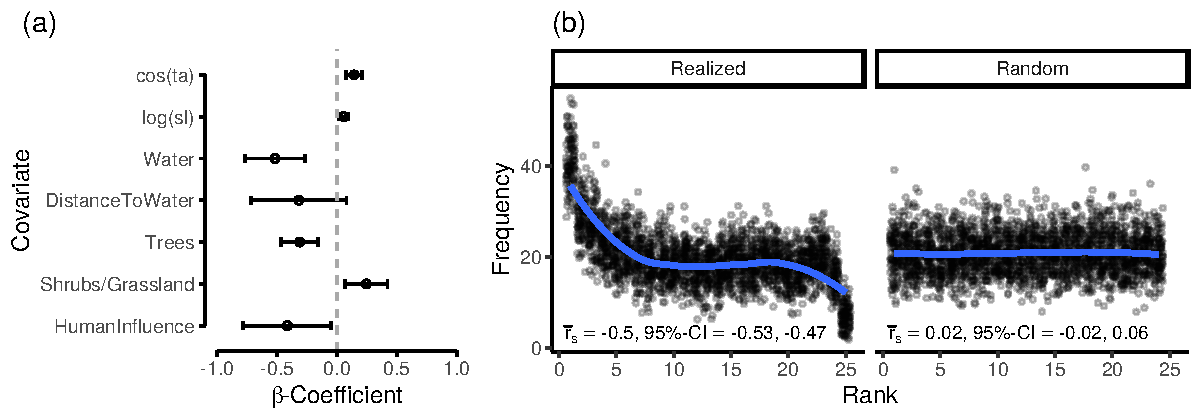
\includegraphics[width = \textwidth]{99_PermeabilityResults.pdf}
    \caption{(a) Estimated selection coefficients from the most parsimonious
    habitat selection model. Negative coefficients indicate avoidance of a
    covariate, positive coefficients selection of a covariate. Whiskers
    delineate the 95\%-CIs for estimated parameters. (b) Results from the k-fold
    cross validation for case-control studies. The left graph shows rank
    frequencies of \textit{realized} steps according to predictions, whereas the
    right graph shows rank frequencies of \textit{randomly selected} steps
    according to predictions. \(\bar{r}_s\) indicates the mean correlation
    coefficient resulting from 100 repetitions of the k-fold cross validation.
    The blue smoothing line was fitted using a locally weighted polynomial
    regression and serves to aid the eye in detecting the trends. Correlation
    coefficients suggest that our prediction was significant and robust,
    evidenced by the fact that the confidence intervals of \(\bar{r}_{s,
    realized}\) and \(\bar{r}_{s, random}\) did overlap and by the fact that
    there was strong and significant correlation between ranks and associated
    frequency for realized steps.}
    \label{PermeabilityResults}
  \end{center}
\end{figure}

Results from the k-fold cross-validation suggested that our prediction was
significant and robust, as highlighted by the fact that the 95\%-CIs intervals
of \(\bar{r}_{s, realized}\) and \(\bar{r}_{s, random}\) did not overlap
(\Cref{PermeabilityResults}b). Likewise, the significant correlation between
ranks and corresponding frequencies for realized steps suggested a good fit
between predictions and observations (\Cref{PermeabilityResults}b).

\subsection{Permeability Surface}
Our prediction of landscape permeability revealed substantial differences across
regions in the study area (\Cref{PermeabilityMap}). Comparisons of median
permeability values (\Cref{PermeabilityComp}) showed that permeability inside
the KAZA-TFCA is more than two times as high as permeability outside it.
Permeability varies by country, with a five-fold permeability difference among
them. Angola and Botswana are characterized by comparably highly permeable
landscapes, Zimbabwe and Zambia are relatively impermeable, and Namibia ranges
in between the two extremes (\Cref{PermeabilityComp}). Visual inspection of our
covariate layers indicated that high permeability in Angola and Botswana is
mainly caused by a combination of low human influences, low tree cover, high
shrubs/grassland cover, and a close distance to water. Although swamps,
wetlands, and permanent water themselves provide little permeability, their
surroundings act as strong attractants to dispersers. The low permeability that
characterizes Zambia and Zimbabwe, on the other hand, is mainly caused by
substantial human influences. Albeit the KAZA-TFCA covers most permeability
hot-spots, several highly permeable regions remain uncovered by its borders.
Across all countries, protected areas provide roughly double the permeability of
unprotected landscapes (\Cref{PermeabilityComp}).

\begin{figure}[hbtp]
  \begin{center}
    \begin{tikzpicture}
        \node[anchor=south west,inner sep=0] (image) at (0,0,0) {
          \begin{minipage}{\textwidth}
            \includegraphics[width = \textwidth]{99_PermeabilityMap.pdf}
          \end{minipage}
        };
        \begin{scope}[x={(image.south east)},y={(image.north west)}]
        \end{scope}
    \end{tikzpicture}
    \caption{Predicted permeability surface for the extent of the KAZA-TFCA.
    Permeability was predicted by calculating selection scores \(w(x) =
    exp(\beta_1 x_1 + \beta_2 x_2 + ... + \beta_n x_n)\) for each raster cell
    based on the raster cell's underlying covariates (\(x_i\)) and estimated
    habitat preferences (\(\beta_i\)). Areas that dispersers find easy to
    traverse are depicted in bright colors. Bold white lines delineate the
    borders of the KAZA-TFCA, whereas dashed white lines show country borders.}
    \label{PermeabilityMap}
  \end{center}
\end{figure}

\begin{table}[h]
  \begin{center}
  \caption{Comparison of median permeability (interquantile range in brackets)
  across countries, separated into areas within and outside the KAZA-TFCA, as
  well as within and outside formally protected areas. High values indicate high
  permeability, whereas low values correspond to low permeability.}
  \label{PermeabilityComp}
  \begin{tabular}{llllll}
    \toprule
    \multicolumn{1}{c}{} & \multicolumn{2}{c}{KAZA-TFCA} &
    \multicolumn{2}{c}{Protection Status} & \multicolumn{1}{c}{} \\
    \cmidrule(l{3pt}r{3pt}){2-3} \cmidrule(l{3pt}r{3pt}){4-5}
    Country & Inside & Outside & Protected & Pastoral & Overall\\
    \midrule
    Angola & 0.36 (0.41) & 0.12 (0.32) & 0.36 (0.41) & 0.12 (0.33) & 0.20 (0.39)\\
    Botswana & 0.25 (0.30) & 0.15 (0.16) & 0.28 (0.35) & 0.15 (0.18) & 0.19 (0.25)\\
    Namibia & 0.22 (0.30) & 0.13 (0.18) & 0.24 (0.30) & 0.11 (0.15) & 0.16 (0.24)\\
    Zambia & 0.05 (0.09) & 0.03 (0.06) & 0.04 (0.10) & 0.03 (0.05) & 0.03 (0.07)\\
    Zimbabwe & 0.07 (0.16) & 0.06 (0.05) & 0.08 (0.17) & 0.05 (0.05) & 0.06 (0.07)\\
    \hline
    Overall & 0.16 (0.30) & 0.07 (0.15) & 0.15 (0.30) & 0.07 (0.15) & 0.10 (0.22)\\
    \bottomrule
  \end{tabular}
  \end{center}
\end{table}

\subsection{Least-Cost Paths \& Least-Cost Corridors}
Our least-cost analysis revealed three major movement corridors of which all
were well-contained within the KAZA-TFCA boundaries (\Cref{LeastCost}). One
major corridor runs SE-NW and connects the Okavango-Linyanti ecosystem in
Botswana with Luengue-Luiana NP in Angola. A second corridor runs W-E between
Chobe NP in Botswana and Zimbabwe's Hwange NP. A third major corridor runs
NE-SW, completely across unprotected areas, and connects Kafue NP in Zambia with
more central regions of the KAZA-TFCA. Several minor corridors branch off from
these three major corridors; these include a southward connection between the
Okavango-Linyanti and the Central Kalahari Game Reserve, a southwesterly
corridor connecting Luengue-Luiana NP with Namibia's Khaudum NP, and a
northeasterly extension of the Hwange corridor into Zimbabwe's Matusadona NP.
According to our predictions, the landscapes in the Okavango-Linyanti region are
the highest frequented dispersal routes within the KAZA-TFCA
(\Cref{LeastCost}b). Our model did not detect any significant direct corridors
between Zimbabwe and Zambia or Zambia and Angola, and only a very limited W-E
direct connection between the Okavango region and Namibia's Khaudum NP. Except
for the corridor into the Central Kalahari National Park, our model did not
detect any significant connectivity outside the boundaries of the KAZA-TFCA.
Furthermore, we found little to no direct connectivity between peripheral
points; that is, most paths and corridors connecting two adjacent peripheral
points run through more central regions before heading towards their destination
at the periphery (\Cref{LeastCost}).

\begin{figure}[hbtp]
  \begin{center}
    \begin{minipage}{0.95\textwidth}
      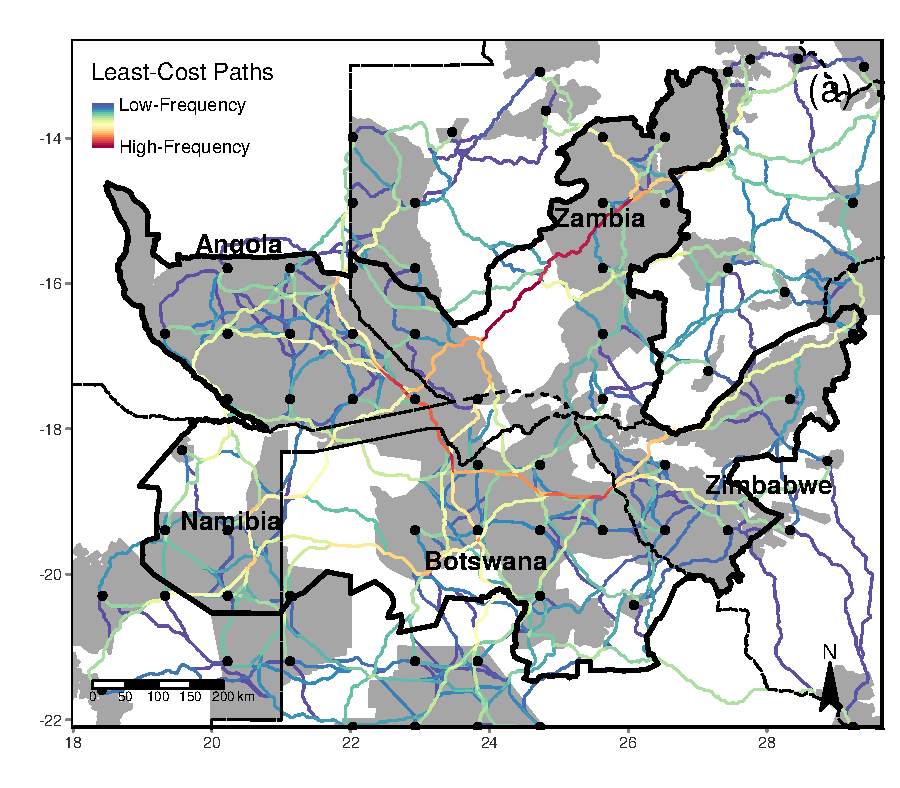
\includegraphics[width = 0.95\textwidth]{99_LeastCostPaths.pdf}
      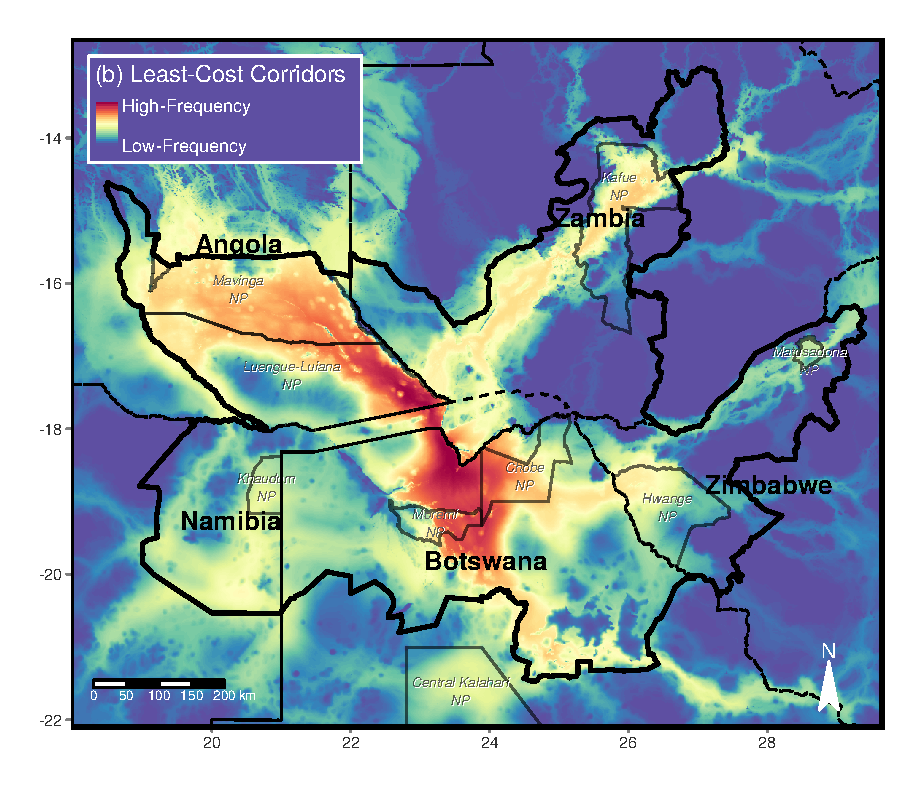
\includegraphics[width = 0.95\textwidth]{99_LeastCostCorrs.pdf}
    \end{minipage}
    \caption{(a) Source points (black dots) and corresponding least-cost paths
    leaving from protected areas (light grey). Note that only contiguous
    protected areas covering more than 700 km\textsuperscript{2} are depicted.
    Continuous thin black lines indicate the borders of the KAZA-TFCA, whereas
    dashed black lines delineate country-borders. (b) Least-cost corridors
    between the same source points as illustrated in subfigure (a). For ease of
    spatial reference, we also labeled some national parks (NPs, in dark-grey).}
    \label{LeastCost}
  \end{center}
\end{figure}

\section{Discussion}
We used GPS relocation data collected on dispersing African wild dogs to
investigate whether their main movement corridors are contained within the
boundaries of the world's largest transboundary conservation area, namely the
KAZA-TFCA. Our analysis suggests that the KAZA-TFCA indeed encompasses all major
corridors of African wild dogs, demonstrating the potential value of such an
initiative. We thus exemplified how pertinent dispersal data of a highly mobile
species can be used to assess the adequacy of already existing or planned
protected areas. Our approach is neither limited to the African wild dog, nor to
our study area and thus applicable to any study system. All covariates used
throughout this study are readily available on a global scale and many of them
are likely to be important determinants of movement behavior, landscape
permeability, and connectivity for other species \citep{Thurfjell.2014,
Zeller.2012}. Interestingly, our predicted network of least cost-paths and
corridors for African wild dogs shows surprising similarities to corridors of
dispersing lions inhabiting the same ecosystem \citep{Elliot.2014,
Cushman.2018}. This not only reinforces confidence in our own predictions but
also suggests potential synergies for the conservation of these two, and
possibly more, species. Expanding our analytical framework to additional species
will likely yield important insights on the consistency of inter-specific
movement corridors, thus highlighting areas that are exceptionally valuable for
the conservation of several species.

Our results emphasize that human influences constitute some of the main barriers
to connectivity among wild dog populations. This conforms to findings on
dispersing wild dogs from eastern Africa \citep{Masenga.2016, Oneill.2020} but
conflicts with findings from South Africa by \cite{DaviesMostert.2012}, who
reported a high willingness of dispersers to cross human-dominated landscapes.
We believe that such differences are due to the unavailability of alternative
routes through natural landscapes, which may have forced dispersers in South
Africa to cross human dominated landscapes despite a strong aversion to do so.
In this regard, our representation of dispersal corridors and the resulting
connectivity appear conservative, as dispersers may be able to make the best out
of a bad situation and cross landscapes characterized by considerably
unfavorable conditions \citep{Palomares.2000, Elliot.2014}. Nevertheless,
successful conservation of this species relies on policymakers' and local
authorities' willingness and ability to provide and conserve natural areas that
remain free from anthropogenic pressures. This is not only paramount in light of
increasing connectivity and facilitating dispersal, but also in terms of
reducing human-caused mortality during dispersal. In fact, previous studies have
shown that human-caused mortality represents a major threat to wild dogs'
ability to disperse \citep{Woodroffe.2019, Cozzi.2020}.

Besides human influences, we identified water as additional obstacle to
dispersal. This corroborates earlier studies showing that water bodies are
almost impenetrable to resident packs \citep{Abrahms.2017} and only infrequently
crossed by dispersing individuals \citep{Cozzi.2020}. An accurate and dynamic
representation of water is thus imperative and particularly relevant in seasonal
or flood-pulsing ecosystems such as the Okavango Delta.

Although dispersers avoided moving through water, they selected locations in its
vicinity. This preference may be caused by the occurence of prey close to water
\citep{Bonyongo.2005}. For the same reason, however, competitors such as lions,
spotted hyenas, and resident wild dogs may also use areas close to water
\citep{Valeix.2010}, thereby occasionally forcing dispersing wild dogs to move
into prey-poorer areas away from water. Given the influence that resident
conspecifics, competitors, and prey can have on dispersers \citep{Cozzi.2018,
Armansin.2019} future studies should strive to collect and incorporate intra-
and interspecific relationships into analyses of landscape connectivity.

Locally, we identified the Okavango-Linyanti region as a potential dispersal hub
through which dispersing wild dogs gain access to more peripheral regions of the
KAZA-TFCA. It appears that the absence of human activities, the central position
within the KAZA-TFCA, and the presence of relatively impermeable water bodies
(e.g. Okavango Delta, Linyanti Swamp) funnel dispersal movements, resulting in a
highly frequented corridor. The key role of the Okavango-Linyanti region for
overall connectivity within the KAZA-TFCA thus calls for actions to secure its
protection status in the future. While the region is currently a Wildlife
Management Area, it has neither the status of a National Park nor that of a Game
Reserve. A similar case of non-formally protected but key dispersal landscape is
represented by the area south of Kafue NP in Zambia, for which a disruption of
its main and narrow dispersal corridor would result in considerable isolation of
its subpopulations. We also revealed a potential southwards corridor between the
Okavango-Linyanti ecosystem and the Central Kalahari National Park.
\cite{Elliot.2014} and \cite{Cushman.2018} identified a similar corridor for
dispersing lions, suggesting that upholding and protecting a link between those
ecosystems is pivotal. Some areas through which the corridor runs are neither
part of the KAZA-TFCA nor profit from any form of protection status. In fact,
human presence and activities along the national road that longitudinally
traverses this corridor may limit realized connectivity \citep{Cozzi.2020}.

Our approach of identifying movement corridors based on pre-defined start and
end points implicitly assumes that individuals know the end point of their
dispersal journey and that they have almost complete knowledge of associated
movement costs \citep{Panzacchi.2016}. Since dispersers often move into unknown
territory, this may not necessarily be the case \citep{Abrahms.2017,
Cozzi.2020}. However, specification of pre-defined end points might not be
necessary, as the parametrized iSSF model can be used as mechanistic movement
model to simulate dispersal events from known source points, yet without
restricting the domain of potential end points \citep{Signer.2017}.
Consequently, movement corridors would emerge more naturally as the result of a
myriad of simulated dispersal events. While a simulation-based approach is
conceptually straightforward, it requires a comprehensive mechanistic
understanding of dispersal movements, which is conditional on our ability to
collect additional dispersal data and adequately represent the landscape through
which individuals move.

Our work shows how dispersal data of a highly mobile species can be used t
identify movement corridors and to assess the adequacy of protected areas. In
our case, the predicted movement corridors of African wild dogs were well
contained within the boundaries of the world's largest transboundary
conservation area, namely the KAZA-TFCA, suggesting that it will significantly
contribute to the long-term viability of this species. Moreover, our
connectivity network allowed revealing potential dispersal hubs through which
dispersers gain access to more remote regions of the study area. Finally, our
investigations showed that human influence constitutes one of the main barriers
to dispersal and substantially reduces landscape connectivity. Successful
conservation of wide-ranging species, such as exemplified by the African wild
dog, will therefore be contingent on the willingness of local authorities,
policymakers, and land managers to preserve areas that remain free from human
strains. Ultimately, our work contributes to the growing field of connectivity
studies and provides and easily expandable framework for assessing the adequacy
of already-existing or planned protected areas.

\section{Authors' Contributions}
D.D.H., D.M.B., A.O. and G.C. conceived the study and designed methodology;
D.M.B., G.C., and J.W.M. collected the data; D.D.H. and D.M.B. analysed the
data; G.C. and A.O. assisted with modelling; D.D.H., D.M.B., and G.C. wrote the
first draft of the manuscript and all authors contributed to the drafts at
several stages and gave final approval for publication.

\section{Data Availability}
GPS movement data of dispersing coalitions will be made available on dryad at
the time of publication.

\section{Acknowledgements}
We thank the Ministry of Environment and Tourism of Botswana for granting
permission to conduct this research. We thank C. Botes, I. Clavadetscher, and G.
Camenisch for assisting with wild dog immobilizations. We also thank B. Abrahms
for sharing her data of three dispersing wild dogs. Furthermore, we are indebted
to Prof. J. Fieberg, who consulted all statistical aspects of this work and P.
Wolski, from the Okavango Research Institute, who assisted us in generating
dynamic water maps. This study was funded by Basler Stiftung für Biologische
Forschung, Claraz Foundation, Idea Wild, Jacot Foundation, National Geographic
Society, Parrotia Stiftung, Stiftung Temperatio, Wilderness Wildlife Trust
Foundation, Forschungkredit der Universität Zürich, and a Swiss National Science
Foundation Grant (31003A\_182286) to A. Ozgul.

\newpage
\begingroup
\singlespacing
\bibliography{Literatur}
\endgroup

\end{document}
